In the following, we write $C(e,e'),M(s,e),EN(s,e)$ to indicate variables
$C_{e,e'},M_{s,e},$ and $EN_{s,e}$ respectively.
\begin{example}
    Consider a firewall where we initially allow all outgoing packets and block all incoming packets.
    We want to allow incoming packets once a packet is sent outside.
    \begin{center}
        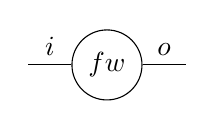
\begin{tikzpicture}[node distance={15mm},main/.style = {draw, circle}]
            \node[main] (s) {$fw$};
            \draw (s) -- node[above]{$i$} (-1,0);
            \draw (s) -- node[above]{$o$} (1,0);
        \end{tikzpicture}
    \end{center}
    We may represent this network with an event structure 
    $\mathrm{E} = (\s{i,o},\e,\vdash)$ where events $o,i$ for incoming 
    and outgoing packets respectively.
    We assume an empty conflict relation and enabling relation
    $\vdash$ the least one that satisfies:
    \begin{align*}
        \e \vdash i, \e \vdash o
    \end{align*}
    The functions of the causal model are as follows:
    \begin{align*}
        \f{M(\e,i)}     & = Min(\e,i) \wedge Con(\e) = Min(\e,i)   \\
                        & = \neg M(\s{o},i)                        \\
        \f{M(\e,o)}     & = Min(\e,o) \wedge Con(\e) =  Min(\e,o)  \\
                        & = \neg M(\s{i},o)                        \\
        \f{M(\s{i},o)}  & = \F                                     \\
        \f{M(\s{o},i)}  & = \F                                     \\
        \f{EN(\e,i)}    & = M(\e,i) \wedge Con(\e) = M(\e,i)       \\
        \f{EN(\e,o)}    & = M(\e,o) \wedge Con(\e) = M(\e,o)       \\
        \f{EN(\s{o},i)} & =
        \left( M(\s{o},i) \vee EN(\e,i)  \right) \wedge Con(\s{o}) \\
                        & = M(\s{o},i) \vee EN(\e,i)               \\
        \f{EN(\s{i},o)} & =
        \left( M(\s{i},o) \vee EN(\e,o) \right)
        \wedge Con(\s{i})                                          \\
                        & = M(\s{i},o) \vee EN(\e,o)               
    \end{align*}
    Now let $\sigma = \s{o}$ be a counterexample.
    Assume that we want to declare $M(\s{i},o) = \F$ as a cause of
    $\sigma \in \mathcal{F}(\mathrm{E})$ using $(\e,\e,\T)$ as a witness.
    First, we need to verify the AC1 condition:
    \begin{align*}
        \m \vDash M(\s{i},o) = \F \wedge \sigma
        \in \mathcal{F}(\vte) \wedge \vec v \in \mathcal{E}
    \end{align*}
    In the actual context we have:
    \begin{align*}
        \m & \vDash EN(\e,i) = \T    \\
        \m & \vDash EN(\s{o},i) = \T \\
        \m & \vDash EN(\e,o) = \T    \\
        \m & \vDash EN(\s{i},o) = \T \\
        \m & \vDash Con(i,o) = \F    
    \end{align*}
    Let $\mathrm{E'} = \vte = (\s{i,o},\e,\vdash')$
    in the actual context so we have:
    \begin{align*}
        \e \vdash' o, \s{i} \vdash' o, \e \vdash' i,
        \s{o} \vdash' i
    \end{align*}
    Which has configurations of the form:
    \begin{center}
        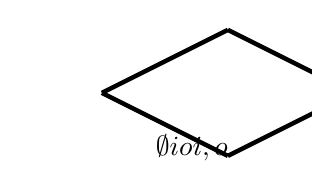
\begin{tikzpicture}[scale=0.8]
            \crd{0}{0}{$\emptyset$}
            \crd[left]{-2}{1}{$\s{i}$}
            \crd[right]{2}{1}{$\s{o}$}
            \crd[right]{0}{2}{$\s{i,o}$}
            \draw [ultra thick] (0,0) -- (2,1);
            \draw [ultra thick] (0,0) -- (-2,1);
            \draw [ultra thick] (-2,1) -- (0,2);
            \draw [ultra thick] (2,1) -- (0,2);
        \end{tikzpicture}
    \end{center}
    It is easy to verify that $\mathrm{E'}$ is an event structure and
    $\sigma$ is a configuration of $\mathrm{E'}$.  
    So, the AC1 condition is satisfied.
    Next, we need to verify the AC2(a) condition:
    \begin{align*}
        \m \vDash [M(\s{i},o) \la T] \sigma \not \in \mathcal{F}(\vte)
        \wedge \vec v \in \mathcal{E}
    \end{align*}
    Assume that we set $M(\s{i},o)$ to true.
    $M(\e,o)$ depends on $M(\s{i},o)$, $E(\e,o)$ depends on $M(\e,o)$, and
    $E(\s{i},o)$ depends on both $M(\s{o},i)$ and $E(\e,i)$
    and these are the only variables that are affected by changing
    $M(\s{i},o)$.
    Thus we have:
    \begin{align*}
        \m & \vDash [M(\s{i},o)\la \T] M(\e,o) = \F     \\
        \m & \vDash [M(\s{i},o)\la \T] EN(\e,o) = \F    \\
        \m & \vDash [M(\s{i},o)\la \T] EN(\s{i},o) = \T
    \end{align*}
    Thus we have:
    \begin{align*}
        \m & \vDash [M(\s{i},o)\la \T]EN(\e,i) = \T    \\
        \m & \vDash [M(\s{i},o)\la \T]EN(\s{o},i) = \T \\
        \m & \vDash [M(\s{i},o)\la \T]EN(\e,o) = \F    \\
        \m & \vDash [M(\s{i},o)\la \T]EN(\s{i},o) = \T \\
        \m & \vDash [M(\s{i},o)\la \T]Con(i,o) = \F
    \end{align*}
    So, if $\mathrm{E}'' = \vte = (\s{i,o},\e, \vdash'')$
    after we have set $M(\s{i},o)$ to true we have:
    \begin{align*}
        \e \vdash'' i, \s{o} \vdash'' i, \s{i} \vdash '' o
    \end{align*}
    Thus configurations of the $\mathrm{E''}$ would be as the right figure
    below:
    \begin{center}
        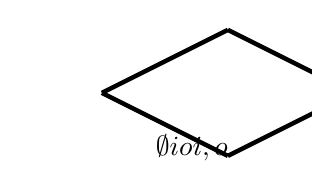
\begin{tikzpicture}[scale=0.8]
            \crd{0}{0}{$\emptyset$}
            \crd[left]{-2}{1}{$\s{i}$}
            \crd[right]{2}{1}{$\s{o}$}
            \crd[right]{0}{2}{$\s{i,o}$}
            \draw [ultra thick] (0,0) -- (2,1);
            \draw [ultra thick] (0,0) -- (-2,1);
            \draw [ultra thick] (-2,1) -- (0,2);
            \draw [ultra thick] (2,1) -- (0,2);
        \end{tikzpicture}
        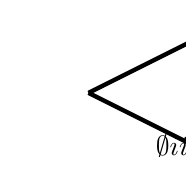
\begin{tikzpicture}[scale=0.8]
            \crd{0}{0}{$\emptyset$}
            \crd[left]{-2}{1}{$\s{i}$}
            \crd[right]{0}{2}{$\s{i,o}$}
            \draw [ultra thick] (0,0) -- (-2,1);
            \draw [ultra thick] (-2,1) -- (0,2);
        \end{tikzpicture}
    \end{center}
    We can easily verify that $\mathrm{E}''$ is an event structure.
    Now, since $\e \not \vdash'' o$, thus $\sigma$ is not a configuration
    of $\mathrm{E}''$.
    So the AC2(a) condition is also satisfied.
    Since we have used an empty $\vec W$ set for the witness, and AC2(a)
    condition is satisfied, thus we can conclude that $M(\s{i},o) = \F$ is a
    cause of $\sigma \in \mathcal{F}(\mathrm{\mathfrak{E}( \vec V)})$.
\end{example}

\begin{example}
    Consider the following network where wish to forward traffic from $a$ to $b$ and $x$ to $y$.
    But, we also want to limit the traffic on the link 3 so that at any moment
    there must be at most one packet traversing this link.
    \begin{center}
        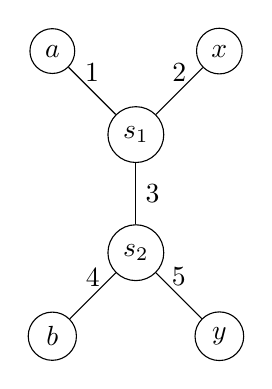
\begin{tikzpicture}[node distance={15mm},main/.style = {draw, circle}]
            \node[main] (s1) {$s_1$};
            \node[main] (s2) [below of=s1] {$s_2$};
            \node[main] (a) [above left of=s1]{$a$};
            \node[main] (x) [above right of=s1]{$x$};
            \node[main] (b) [below left of=s2]{$b$};
            \node[main] (y) [below right of=s2]{$y$};
            \draw (a) --  node[above]{1} (s1);
            \draw (x) --  node[above]{2}(s1);
            \draw (s1) --  node[right]{3}(s2);
            \draw (b) --  node[above]{4}(s2);
            \draw (y) --  node[above]{5}(s2);
        \end{tikzpicture}
    \end{center}
    We define events $a,x,b,y$ representing the forwarding of a packet from
    1 to 3, 2 to 3, 3 to 4, and 3 to 5 respectively.
    We define an event $c$ when congestion is detected on link 3 (at least two packets are being traversed through the link).
    We define the conflict relation in such a way that we have:
    \begin{align*}
        a \# y, x\# b
    \end{align*}
    We consider an enabling relation the least one for which we have:
    \begin{align*}
        \e \vdash a, \e \vdash x, \s{a} \vdash b, \s{x} \vdash y,
        \s{a,x} \vdash c
    \end{align*}
    Assume that $\sigma = \s{a,x,c}$ is given as a counterexample.
    Let $\mathrm{E'} = \vte$, so we wish to find the cause of
    $ \sigma \in \mathcal{F}(E')$.
    Configurations of $\mathrm{E'}$ are as follows:
    \begin{center}
        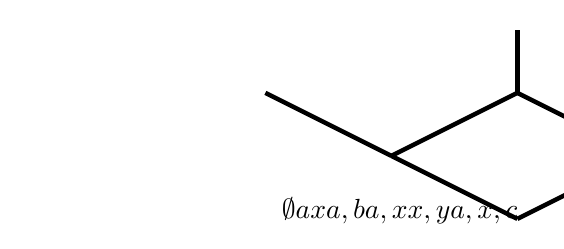
\begin{tikzpicture}[scale=0.8]
            \crd{0}{0}{$\emptyset$}
            \crd[above]{-2}{1}{$\s{a}$}
            \crd[above]{2}{1}{$\s{x}$}
            \crd[left]{-4}{2}{$\s{a,b}$}
            \crd[left]{0}{2}{$\s{a,x}$}
            \crd[left]{4}{2}{$\s{x,y}$}
            \crd[left]{0}{3}{$\s{a,x,c}$}
            \draw [ultra thick] (0,0) -- (-2,1);
            \draw [ultra thick] (0,0) -- (2,1);
            \draw [ultra thick] (-2,1) -- (-4,2);
            \draw [ultra thick] (-2,1) -- (0,2);
            \draw [ultra thick] (2,1) -- (0,2);
            \draw [ultra thick] (2,1) -- (4,2);
            \draw [ultra thick] (0,2) -- (0,3);
        \end{tikzpicture}
    \end{center}
    Obviously, $\sigma$ is a configuration of $\mathrm{E'}$.
    Now, let's consider $C(a,x) = \F$ as a cause using the witness
    $(\e,\e,\T)$.
    Now let $\mathrm{E}'' = \vte = (E, \#'',\vdash'')$ after we set $C(a,x)$ to true. So we have $a\#''x$ and $x\#''a$.
    First, note that $C(a,x)$ only affects terms like $Con(s)$ 
    where $ \s{a,x} \subseteq s$ which in turn only affects 
    variables of the form $M(s,e)$ or $EN(s,e)$.
    So, we can safely conclude that changing $C(a,x)$ has no effect
    on $M_{\e,a},M_{\e,x},M_{\s{a},b},M_{\s{b},a}$ as well as
    $EN_{\e,a},EN_{\e,x},EN_{\s{a},b},EN_{\s{b},a}$.
    Thus we have:
    \begin{align*}
        \e \vdash'' a, 
        \e \vdash'' x, 
        \s{a} \vdash'' b, 
        \s{x} \vdash'' y \\
        a\#''y,y\#''a,x\#''b,b\#''x,a\#''x, x\#''a
    \end{align*}
    So, the configurations of $\mathrm{E}''$ have the form:
    \begin{center}
        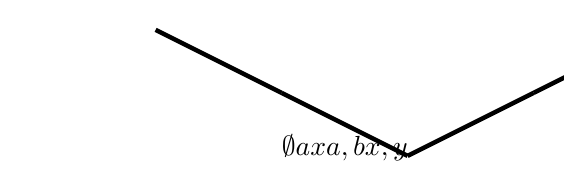
\begin{tikzpicture}[scale=0.8]
            \crd{0}{0}{$\emptyset$}
            \crd[above]{-2}{1}{$\s{a}$}
            \crd[above]{2}{1}{$\s{x}$}
            \crd[left]{-4}{2}{$\s{a,b}$}
            \crd[left]{4}{2}{$\s{x,y}$}
            \draw [ultra thick] (0,0) -- (-2,1);
            \draw [ultra thick] (0,0) -- (2,1);
            \draw [ultra thick] (-2,1) -- (-4,2);
            \draw [ultra thick] (2,1) -- (4,2);
        \end{tikzpicture}
    \end{center}
    In the new event structure, $\sigma$ is no longer a configuration, thus $AC2(a)$ is satisfied.
    Since we have used an empty $\vec W$ in the witness and AC1 and AC2(a)
    are satisfied, thus we can conclude that $C(a,x) = \F$ is a cause of
    $\sigma \in \mathcal{F}(\mathrm{E}')$


\end{example}

\begin{example}
    Consider the following network where we have
    a stateful firewall on the switch $s$.
    Initially, we allow outgoing packets from $a$ and
    block all incoming packets from either $b$ or $c$.
    Assume that packets from $a$ are broadcasted to
    both $b$ and $c$ and we wish to allow traffic
    from both of them afterward.
    \begin{center}
        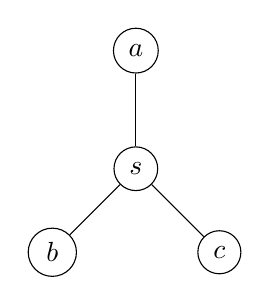
\begin{tikzpicture}[node distance={15mm},main/.style = {draw, circle}]
            \node[main] (s) {$s$};
            \node[main] (a) [above of=s] {$a$};
            \node[main] (b) [below left of=s] {$b$};
            \node[main] (c) [below right of=s] {$c$};
            \draw (s) -- (a);
            \draw (s) -- (b);
            \draw (s) -- (c);
        \end{tikzpicture}
    \end{center}
    We define an event structure where
    $\mathcal{E} = \s{a,b,c,i}$.
    We let $a,b,c$ to represent the events of sending
    a packet from $a$,$b$ and $c$ to $s$ respectively.
    Let $i$ indicate the event of the forwarding of
    an arbitrary packet from $s$ to $a$ (this may coming
    from either $b$ or $c$).
    We consider an empty conflict relation and enabling
    relation the least one for which we have:
    \begin{align*}
        \e \vdash a,\e \vdash b, \e \vdash c,
        \s{b} \vdash i, \s{c} \vdash i
    \end{align*}
    We may consider the configuration $\sigma = \s{b,c,i}$ as a
    counterexample since $i$ is happened while $a$ has not been happened yet.
\end{example}